\documentclass[titlepage,12pt]{article}

\usepackage[T2A]{fontenc}
\usepackage[cp1251]{inputenc}  

\usepackage{amsmath}
\usepackage{amssymb}
\usepackage{graphicx}
\renewcommand{\figurename}{Рис.}

\oddsidemargin = 0.6cm
\textwidth = 16cm
\textheight = 21cm
\headheight = 0cm
\sloppy

\author{Кочуркин Иван Алексеевич\\ Группа ИУ7-92 \\ Вариант \textnumero 11}
\title{Отчёт по лабораторной работе \textnumero 1 \\по курсу\\ Методы вычислений}
\date{2011 г.}

\begin{document}

\maketitle

\section{Постановка задачи}
\subsection{Формулировка задачи}

Найти температуру $u(x,t)$ тонкого стержня длиной $l$ с теплоизолированной боковой поверхностью, на концах которого задан температурный режим. Коэффициент теплопроводности $K$ меняется в зависимости от температуры по заданному закону \( K=K(u) \). В начальный момент времени \( t=0 \) стержень находится при фиксированной температуре $u_0$ по всей длине. Найти момент времени $T$, в который температура в середине стержня будет максимальной.

\subsection{Исходные данные}
\begin{enumerate}
	\item{Длина стержня \(l = 1\)}
	\item{Плотность массы \(den = 1\)}
	\item{Удельная теплоёмкость стержня \(c = 0.5\)}
	\item{Начальная температура стержня \(u_0 = 0.1\)}
	\item{Постоянные: \(a = 0.1\), \(b = 1\), \(\sigma = 2\)}
	\item{Коэфициент теплопроводности \(K(u) = a + bu^\sigma = 0.1 + 1*u^{2}\)}
	\item{Начальное распределение температуры \(\varphi (x) \equiv u_0\)}
	
	\item{Температура на правом конце стержня фиксированна и равна \(u_0\)}
	
		\item{Тепловой поток на левом конце стержня}
	\begin{equation}
	W_3(t) = \begin{cases}
							2Q (t_0-t), &\text{$0 \leqslant t < t_0$}\\ 
							0, &\text{$t_0 \leqslant t$}
				 			\end{cases}
	\end{equation}
	
	\item{\(t_0 = 0.5\), \(Q = 10\)}
\end{enumerate}

\setcounter{page}{2}
\newpage
\section{Теоретические сведения}
\subsection{Краевая задача}

\begin{displaymath}
\left \{ 
\begin{array}{ll}
c\rho \frac{\partial u}{\partial t} = \frac{\partial }{\partial x}\left(K(u)\frac{\partial u}{\partial x}\right),\quad x \in (0;L), \quad t > 0
 & \\
u(x,0) = u_0 & \\
\left.K(u)\frac{\partial u}{\partial x}\right |_{x=0} = W_4(t) \\
\left.K(u)\frac{\partial u}{\partial x}\right |_{x=l} = 0
\end{array} 
\right.
\end{displaymath}

\subsection{Разностная схема}
Для численного решения данной краевой задачи используется неявная разностная схема.
 
Введём сетку $W_t^\tau$ с узлами \(w_i^j = (x_i, t_j)\), \(i = \overline{0:N}\), \(j = \overline{0:M}\); где \(x_i = ih\), \(t = j\tau\) 

Используем неявную схему:
\begin{equation}
\frac{u_i^{j+1} - u_i^j}{\tau} = \frac{K_{i+}^{j+1}(u_{i+1}^{j+1} - u_i^{j+1}) - K_{i-}^{j+1}(u_i^{j+1} - u_{i-1}^{j+1})}{h^2}
\end{equation}

где
\begin{equation}
K_{i+}^{j+1} = \frac{K_{i+1}^{j+1} + K_i^{j+1}}{2};   \qquad
K_{i-}^{j+1} = \frac{K_i^{j+1} + K_{i-1}^{j+1}}{2} 
\end{equation}

Преобразовывая уравнение получаем:
\begin{equation}
u_i^j = (1 + \alpha(K_{i+}^{j+1} + K_{i-}^{j+1}))u_i^{j+1} - \alpha{K_{i+}^{j+1}u_{i+1}^{j+1}} - \alpha{K_{i-}^{j+1}u_{i-1}^{j+1}}; 
\end{equation}

Следовательно:
\begin{equation}
u_i^j = a_iu_{i-1}^{j+1} + b_iu_i^{j+1} +c_iu_{i+1}^{j+1}; 
\end{equation}

где

\begin{displaymath}
a_i = -\alpha{K_{i-}^{j+1}};   \qquad
b_i = (1 + \alpha{(K_{i+}^{j+1} + K_{i-}^{j+1})});   \qquad
c_i = - \alpha{K_{i+}^{j+1}};   \qquad
\alpha = \frac{\tau}{h^2};
\end{displaymath}

Начальное условие: \(u_i^0 = u_0\).

Граничные условия:
\begin{equation}
K_{0+}^{j+1}\frac{u_1^{j+1} - u_0^{j+1}}{h} = W|_{x=0} = W_3(t);  \qquad
u = u_0;
\end{equation}

Следовательно:
\begin{equation}
u_1^{j+1} - u_0^{j+1} = \frac{W_3h}{K_{0+}^{j+1}};   \qquad
u = u_0;
\end{equation}

Тогда для \(j+1\)-го слоя получим уравнение \(Au^{j+1} = F\)

Где
\begin{displaymath}
 A = \left( \begin{array}{ccccccc}
-1 & 1 & 0 & 0 & ... & 0 & 0 \\
a_1 & b_1 & c_1 & 0 & ... & 0 & 0 \\
0 & a_2 & b_2 & c_2 & ... & 0 & 0 \\
0 & 0 & a_3 & b_3 & ... & 0 & 0 \\
. & . & . & . & . & . & . \\
0 & 0 & 0 & 0 & ... & b_{N-1} & 0 \\
0 & 0 & 0 & 0 & ... & 0 & 1 \\
\end{array}
\right)  \qquad
 F = \left( \begin{array}{c}
\frac{W_3^{j+1}h}{K_{0+}^{j+1}}  \\
f_1 \\
f_2 \\
f_3 \\
... \\
f_{N-1} \\
u_0  \\
\end{array}
\right) 
\end{displaymath}

\subsection{Устойчивость}
Условие устойчивости для параметрической схемы с параметром $\alpha$  и \(K = K(u(x))\)

\begin{equation}
(\frac{1}{2} - \alpha)\max_{0\le x \le l}K(u(x))\frac{\tau}{h^2} \le 1
\end{equation}
 
Для неявной схемы это условие выполняется при любых соотношениях $h$  и $\tau$ .

\subsection{Аппроксимация}
Выбранная разностная схема имеет порядок аппроксимации $O(\tau + h^2)$ для ДУ и $O(h)$  - для граничных условий.

\newpage
\section{Результаты}

\begin{figure}[h]
\centering
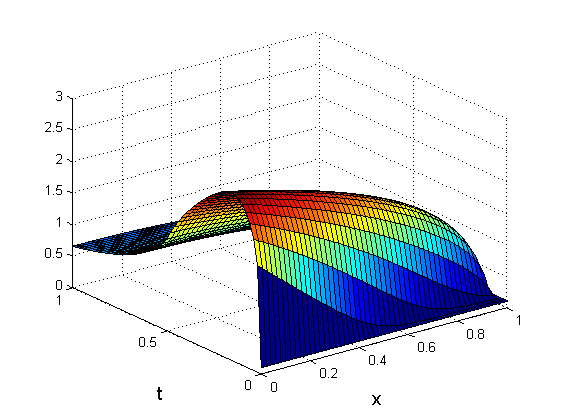
\includegraphics[width = 16cm]{Screen.png}
\caption{Температурное поле}
\label{fig:16}	
\end{figure}

\end{document}
